\documentclass{beamer}
\usetheme{Madrid}
%\usecolortheme{beaver}
\usepackage[utf8x]{inputenc}
\usepackage[serbian]{babel}
\usepackage{verbatim}
\usepackage{amsmath}
\usepackage{graphicx}
\usepackage{caption}
\usepackage{pgfplots}
\pgfplotsset{compat=1.3}

\pgfplotsset{%
    % #1: index in the group(0,1,2,...)
    % #2: number of plots of that group
    bar group size/.style 2 args={%
        /pgf/bar shift={%
                % total width = n*w + (n-1)*skip
                % -> subtract half for centering
                -0.5*(#2*\pgfplotbarwidth + (#2-1)*\pgfkeysvalueof{/pgfplots/bar group skip})  +
                % the '0.5*w' is for centering
                (.5+#1)*\pgfplotbarwidth + #1*\pgfkeysvalueof{/pgfplots/bar group skip}},%
    },
    bar group skip/.initial=2pt,
    plot 0/.style={blue,fill=blue!30!white,mark=none},%
    plot 1/.style={red,fill=red!30!white,mark=none},%
    plot 2/.style={brown!60!black,fill=brown!30!white,mark=none},%
    plot 3/.style={gray,fill=gray,mark=none},%
}

\title{GraalVM}
\subtitle{predmet: Metodologija stručnog i u naučnog rada}
\author{Bojan Bardžić \and Milica Gnjatović \and Pavle Savić \and Andrija Urošević}
\institute{Matematički fakultet}
\date{}

\usepackage{fancyhdr}

\begin{document}
	\begin{frame}
		\titlepage
	\end{frame}
	
	\section{Uvod}
	\begin{frame}
		\frametitle{Uvod}
		
		\begin{figure}
			\begin{center}
				
\includegraphics[width=0.5\linewidth]{imgs/graalvm_logo.png}	
			\end{center} 
		\end{figure}
	
		\center	
		\textit{high-performance JDK distribution written for Java and other JVM languages}

		\begin{flushleft}
			\begin{itemize}
				\item \emph{One VM to rull them all}
				\item Oracle Labs
				\item Community i Enterprise Edition
				\item JVM + JDK	
				\item JIT i AOT
			\end{itemize}
		\end{flushleft}


	\end{frame}

	\begin{frame}
		\frametitle{Podržani jezici}
		\begin{figure}
			
\includegraphics[width=0.16\linewidth]{imgs/java_logo.png}
			
\includegraphics[width=0.16\linewidth]{imgs/c_logo.png}
			
\includegraphics[width=0.16\linewidth]{imgs/cpp_logo.png}
			
\includegraphics[width=0.16\linewidth]{imgs/r_logo.png}
			
\includegraphics[width=0.16\linewidth]{imgs/python_logo.png}
			
\includegraphics[width=0.16\linewidth]{imgs/ruby_logo.png}
			
\includegraphics[width=0.16\linewidth]{imgs/js_logo.png}
			
\includegraphics[width=0.16\linewidth]{imgs/nodejs_logo.png}
			
\includegraphics[width=0.16\linewidth]{imgs/clojure_logo.png}
			
\includegraphics[width=0.16\linewidth]{imgs/kotlin_logo.png}
			
\includegraphics[width=0.16\linewidth]{imgs/scala_logo.png}
			
\includegraphics[width=0.16\linewidth]{imgs/wa_logo.png}
		\end{figure}
		
		\begin{flushleft}
			\begin{itemize}
				\item Eclipse, NetBeans, IntelliJ IDEA i Visual Studio Code
				\item Windows, Linux, MacOS
			\end{itemize}
		\end{flushleft}
		
	
	\end{frame}	
	

	\section{Šta obuhvata projekat?}
	
	\begin{frame}
		\frametitle{Zamena za JVM}
		\begin{itemize}
			\item Može se koristiti umesto JVM
			\item Za Ruby do 30\% brži
			\item Za Javu sličan HotSpot VM
			\item Pisan u Javi
			\item Veliki potencijal za optimizaciju
		\end{itemize}
	\end{frame}	
	
	\begin{frame}
		\frametitle{Native Image}
		\begin{itemize}
			\item AOT kompajler za Javu
			\item Mikroservisi na cloud-u
			\item Manje zauzeće memorije
			\item Brže izvršavanje
			\item Ne može se primeniti na sve Java programe
		\end{itemize}
	\end{frame}	
	
	
	\begin{frame}
		\frametitle{Truffle}
		 \begin{itemize}
			\item Omogućava pravljenje alata i interpretera
			\item Parcijalna evaluacija
			\item Podrška za Ruby, R, Python
			\item Podrška za LLVM jezike
			\item Omogućava poliglotsko programiranje
		 \end{itemize}
	\end{frame}	

	\begin{frame}
		\frametitle{Espresso - Java on Truffle}

		\begin{figure}
			\begin{center}
				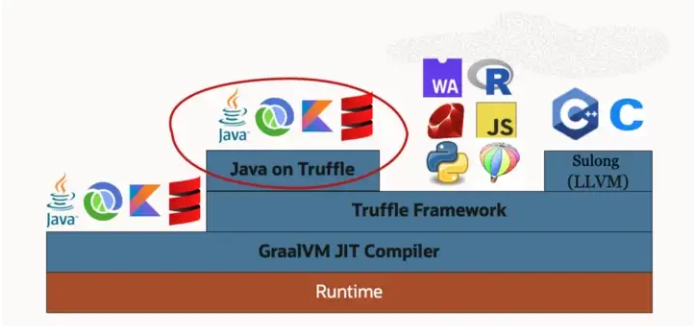
\includegraphics[width=0.5\linewidth]{imgs/java_on_truffle.png}	
			\end{center} 
		\end{figure}

		\center	
		\textit{Java on Truffle u GraalVM ekosistemu}


		\begin{flushleft}
			\begin{itemize}
				\item Dostupna od verzije 21.0
				\item Implementacija JVM specifikacije pomoću Truffle-a
				\item Interoperabilnost sa interpretiranim i LLVM jezicima
				\item \emph{Self-hosting}, metacirkularna VM
				\item Izvorni kod razumljiv Java programerima
				\item Istovremeno JVM i Java program
			\end{itemize}
		\end{flushleft}

	\end{frame}	

	\begin{frame}
		\frametitle{Espresso - Java on Truffle}

		\begin{flushleft}
			\begin{itemize}
				\item Moguće ugraditi Java 8 kontekst u Java 11 aplikaciju
				\item Povećana izolovanost \emph{host} VM-a i Java programa
				\item Napredni \emph{hot swap} prilikom debagovanja
				\item Eksperimentalna tehnologija
			\end{itemize}
		\end{flushleft}


		\begin{figure}
			\begin{center}
				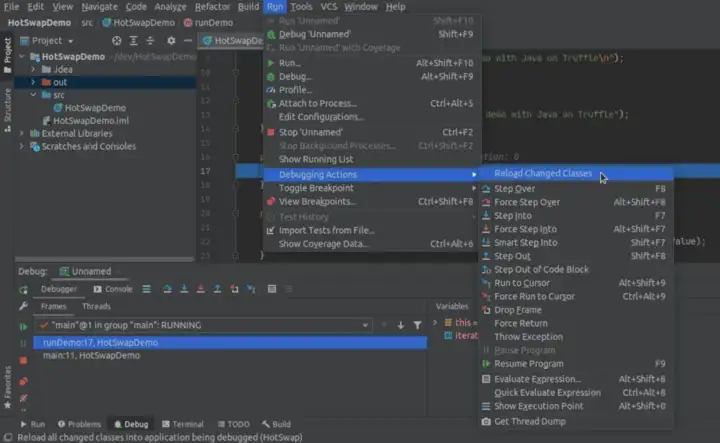
\includegraphics[width=0.5\linewidth]{imgs/hotswap.png}	
			\end{center} 
		\end{figure}

		\center	
		\textit{Hot Swap u IntelliJ IDEA debageru}

	\end{frame}
	
		
	\section{Karakteristike}
	
	\begin{frame}
		\frametitle{Visoke performanse}

        \begin{figure}[scale=0.5]
            \begin{center}
                \begin{tikzpicture}[scale=0.7]
                    \begin{axis}[
                            width=0.85\textwidth,
                            x tick label style={/pgf/number format/1000 sep=},
                            ylabel=Prosečno vreme u milisekundama $(ms)$,
                            enlargelimits=0.15,
                            legend style={at={(0.5,-0.15)},
                            anchor=north,legend columns=-1},
                            ybar,
                            bar width=7pt,
                            xtick={0,1,2,3,4,5},
                            xticklabels={h2, lusearch, xalan, pmd, sunflow, jython},
                        ]
                        \addplot[plot 0,bar group size={0}{4}]
                        coordinates {(0,4494.95) (1,2683.40) (2,863.32) (3,138.23) (4,5062.05) (5,6652.86)};
                        \addplot[plot 1,bar group size={1}{4}]
                        coordinates {(0,5327.10) (1,2757.10) (2,277.41) (3,194.61) (4,5626.25) (5,7038.34)};
                        \addplot[plot 2,bar group size={2}{4}]
                        coordinates {(0,10821.85) (1,2874.50) (2,870.72) (3,201.95) (4,5417.25) (5,6433.60)};
                        \addplot[plot 3,bar group size={3}{4}]
                        coordinates {(0,9550.05) (1,2886.15) (2,232.51) (3,276.76) (4,6151.25) (5,6672.10)};
                        \legend{GraalVM EE, GraalVM CE, JDK10, JDK11}
                    \end{axis}
                \end{tikzpicture}
            \end{center}
            \caption{\emph{DaCapo} benčmark na \emph{GraalVM EE, GraalVM CE, JDK10, JDK11}.}
            \label{fig:dacapo}
        \end{figure}


    \end{frame}	

    \begin{frame}
        \frametitle{Poliglot programiranje}
        \begin{itemize}
            \item Svi jezici imaju prednosti u nekom domenu problema
            \item Koristimo odgovarajući jezik za rešavanje određenog problema
            \item Integrišemo više programskih jezika u jedan projekat
            \item GraalVM rešava problem integrisanja više programskih jezika
            \item TruffleVM
        \end{itemize}
	\end{frame}	

	\begin{frame}
		\frametitle{Napredni alati}
        \begin{table}
            \centering
            \begin{tabular}{|l|l|}
                \hline
                VS Code Extensions & Radno okruženje unutar VS Code-a\\
                \hline
                GraalVM Dashboard & Vizuelna reprezentacija delova projekta\\
                \hline
                Chrome Debugger & Debager za JS, Ruby, R i Python\\
                \hline
                VisualVM & Profajler, monitor, aktivne niti\ldots\\
                \hline
                GraalVM Insight & Praćenje programa u izvršavanju\\
                \hline
                Ideal Graph Visualizer & Graf faza kompilacija\\
                \hline
            \end{tabular}
            \caption{Napredni alati unutar Projekta \emph{GraalVM}.}\label{alati}
        \end{table}
	\end{frame}	

	\section{Zaključak}
	
	\begin{frame}
		\frametitle{Ko koristi GraalVM?}
		\begin{figure}
			
\includegraphics[width=0.2\linewidth]{imgs/facebook.png}
			
\includegraphics[width=0.25\linewidth]{imgs/twitter.png} 
			
\includegraphics[width=0.25\linewidth]{imgs/nvidia.png} \\
			
\includegraphics[width=0.25\linewidth]{imgs/gs.png}
			
\includegraphics[width=0.25\linewidth]{imgs/politie.png}
			
\includegraphics[width=0.25\linewidth]{imgs/oracle.png}
		\end{figure}
	\end{frame}
	
	\begin{frame}
		\center	
		\textit{Hvala na pažnji!}
	\end{frame}

	\begin{frame}
		\nocite{*}
		\bibliography{GraalVM} 
		\bibliographystyle{abbrv}
	\end{frame}
	
\end{document}
